% =====================================================================
%  SDG Nexus — Minor Project Report
%  Format: DBUU B.Tech project report (Department of CSE, SoEC)
%  Compile on Overleaf with pdfLaTeX (Menu -> Compiler -> pdfLaTeX).
% =====================================================================
\documentclass[12pt,a4paper,oneside]{report}

% ---------- Page layout & fonts ----------
\usepackage[a4paper,left=1.25in,right=1in,top=1in,bottom=1in]{geometry}
\usepackage[T1]{fontenc}
\usepackage[utf8]{inputenc}
\usepackage{lmodern}
\usepackage{setspace}
\onehalfspacing
\setlength{\parskip}{4pt}

% ---------- Packages ----------
\usepackage{graphicx}
\usepackage{float}
\usepackage{amsmath,amssymb}
\usepackage{array,tabularx,booktabs,longtable,multirow}
\usepackage[table]{xcolor}
\usepackage{enumitem}
\usepackage{caption}
\usepackage{titlesec}
\usepackage{tocloft}
\usepackage{tikz}
\usetikzlibrary{arrows.meta,positioning,shapes.geometric,shapes.multipart,fit,calc,backgrounds,shadows}
\usepackage{pgfgantt}
\usepackage{listings}
\usepackage[hidelinks]{hyperref}

% ---------- Colours used in diagrams ----------
\definecolor{nexusblue}{HTML}{1F4E79}
\definecolor{nexusgreen}{HTML}{3F7F3F}
\definecolor{nexusamber}{HTML}{B7791F}
\definecolor{nexusred}{HTML}{A33A3A}
\definecolor{nexusgrey}{HTML}{F2F2F2}
\definecolor{nexusline}{HTML}{555555}

% ---------- Chapter heading: "CHAPTER 1" / "INTRODUCTION" (centred) ----------
\titleformat{\chapter}[display]
  {\normalfont\bfseries\centering}
  {\Large CHAPTER \thechapter}
  {6pt}
  {\Large\MakeUppercase}
\titlespacing*{\chapter}{0pt}{0pt}{24pt}
\titleformat{\section}{\normalfont\large\bfseries}{\thesection}{0.8em}{}
\titleformat{\subsection}{\normalfont\normalsize\bfseries}{\thesubsection}{0.8em}{}

% ---------- Table of contents styling ----------
\renewcommand{\contentsname}{\centering TABLE OF CONTENTS}
\renewcommand{\listfigurename}{\centering LIST OF FIGURES}
\renewcommand{\listtablename}{\centering LIST OF TABLES}
\setcounter{tocdepth}{1}   % chapters and sections only, as in the prescribed format
\renewcommand{\cftchappresnum}{CHAPTER }
\renewcommand{\cftchapaftersnum}{:}
\setlength{\cftchapnumwidth}{6.2em}
\renewcommand{\cftchapleader}{\cftdotfill{\cftdotsep}}
\renewcommand{\cftfigpresnum}{Figure }
\setlength{\cftfignumwidth}{5.6em}
\setlength{\cftfigindent}{0pt}
\renewcommand{\cfttabpresnum}{Table }
\setlength{\cfttabnumwidth}{5.2em}
\setlength{\cfttabindent}{0pt}

% ---------- Captions ----------
\captionsetup{font=small,labelfont=bf,labelsep=space}
\captionsetup[figure]{name=Figure}
\captionsetup[table]{name=Table,position=top}

% ---------- Lists ----------
\setlist{itemsep=2pt,topsep=4pt}

% ---------- Code listings ----------
\lstset{basicstyle=\ttfamily\footnotesize,breaklines=true,frame=single,columns=fullflexible}

% ---------- Project details (edit here) ----------
\newcommand{\projecttitle}{SDG Nexus: A Collaborative Platform Connecting Community Problems, Universities and CSR Funding for Verified SDG Impact}
\newcommand{\shorttitle}{SDG Nexus}
\newcommand{\guide}{Dr.\ Deepa Bhatt}
\newcommand{\guidedesignation}{Assistant Professor}
\newcommand{\hod}{Mr.\ Dhajvir Singh Rai}
\newcommand{\submissiondate}{NOVEMBER 2026}

\begin{document}

% =====================================================================
%  FRONT MATTER (roman page numbers)
% =====================================================================
\pagenumbering{roman}
% =====================================================================
%  TITLE PAGE  (page i, number not shown)
% =====================================================================
\begin{titlepage}
\begin{center}
\thispagestyle{empty}
{\large A Project Report on}\\[0.6cm]
{\Large\bfseries \projecttitle}\\[0.9cm]
{\normalsize Submitted in the Partial Fulfilment of the Requirements for the Degree of}\\[0.3cm]
{\large\bfseries BACHELOR OF TECHNOLOGY}\\[0.2cm]
{\normalsize in}\\[0.2cm]
{\large\bfseries COMPUTER SCIENCE \& ENGINEERING}\\[0.6cm]
{\normalsize by}\\[0.3cm]
{\normalsize
Yashpal Singh Rajwar (24BTCSEAI0107)\\
Nitin Saini (24BTCSE0160)\\
Saifullah Ahad (24BTCSEAI0144)\\
Muzamil Akbar Dar (24BTCSEAI0020)\\}
\vspace{0.6cm}
{\normalsize Under the supervision of}\\[0.2cm]
{\normalsize\bfseries \guide}\\
{\normalsize \guidedesignation}\\[0.7cm]

\includegraphics[width=3.2cm]{figures/dbuu-logo.png}\\[0.6cm]
{\normalsize\bfseries Department of Computer Science and Engineering}\\
{\normalsize School of Engineering \& Computing (SoEC)}\\[0.2cm]
{\normalsize\bfseries DEV BHOOMI UTTARAKHAND UNIVERSITY, UTTARAKHAND-248001}\\[0.4cm]
{\normalsize\bfseries \submissiondate}
\end{center}
\end{titlepage}
\setcounter{page}{2}

% =====================================================================
%  CANDIDATE'S DECLARATION  (ii)
% =====================================================================
\chapter*{CANDIDATE'S DECLARATION}
\addcontentsline{toc}{chapter}{Candidate's Declaration}
We hereby declare that the work presented in this project titled, ``\projecttitle'' submitted by us in the partial fulfilment of the requirement of the award of the degree of Bachelor of Technology (B.Tech.) submitted in the Department of Computer Science \& Engineering, Dev Bhoomi Uttarakhand University, Dehradun, is an authentic record of our work carried out under the guidance of \guide, \guidedesignation, Department of Computer Science and Engineering under SoEC, Dev Bhoomi Uttarakhand University, Dehradun.

\vspace{0.8cm}
\noindent Date: \rule{3cm}{0.4pt}

\vspace{0.6cm}
\noindent
\begin{tabularx}{\textwidth}{@{}XX@{}}
\textbf{Yashpal Singh Rajwar} & \textbf{Nitin Saini} \\
B.Tech (CSE) & B.Tech (CSE) \\
Roll No.: 24BTCSEAI0107 & Roll No.: 24BTCSE0160 \\[0.9cm]
\textbf{Saifullah Ahad} & \textbf{Muzamil Akbar Dar} \\
B.Tech (CSE) & B.Tech (CSE) \\
Roll No.: 24BTCSEAI0144 & Roll No.: 24BTCSEAI0020 \\
\end{tabularx}

\vspace{0.4cm}
\noindent Dev Bhoomi Uttarakhand University, Dehradun

\vspace{1.4cm}
\noindent\textbf{Approved By} \hod\\
Head of the Department\\
(Computer Science \& Engineering)\\
Dev Bhoomi Uttarakhand University, Dehradun

% =====================================================================
%  CERTIFICATE  (iii)
% =====================================================================
\chapter*{CERTIFICATE}
\addcontentsline{toc}{chapter}{Certificate}
It is to certify that the Project entitled ``\projecttitle'' which is being submitted by Yashpal Singh Rajwar (24BTCSEAI0107), Nitin Saini (24BTCSE0160), Saifullah Ahad (24BTCSEAI0144) and Muzamil Akbar Dar (24BTCSEAI0020) to Dev Bhoomi Uttarakhand University, Dehradun, in the fulfilment of the requirement for the award of the degree of Bachelor of Technology (B.Tech.) is a record of bonafide work carried out by them under my guidance and supervision. The matter presented in this project has not been submitted either in part or full to any University or Institute for award of any degree.

\vspace{2.5cm}
\noindent\textbf{\guide}\\
\guidedesignation\\
Department of Computer Science and Engg.\\
Dev Bhoomi Uttarakhand University, Dehradun\\
(Uttarakhand) INDIA

% =====================================================================
%  ABSTRACT  (iv)
% =====================================================================
\chapter*{ABSTRACT}
\addcontentsline{toc}{chapter}{Abstract}
Every district in India has documented local problems---contaminated drinking water, failing health-centre equipment, school dropouts, flooded roads. Three groups that could solve them rarely meet: citizens who report problems through grievance portals but seldom see a resolution, universities whose students build semester projects on hypothetical problems, and companies that spend their mandatory Corporate Social Responsibility (CSR) budgets with little visibility into actual outcomes. The missing piece is not resources or expertise but a trustworthy way of routing each problem to the people who can solve and fund it, and of proving that the solution was delivered.

This project presents \textbf{SDG Nexus}, a web platform that turns a citizen's report into a funded, student-built and verified solution aligned to the United Nations Sustainable Development Goals (SDGs). A citizen reports a problem with location and photographs; a district officer verifies it; the platform tags the relevant SDGs and suggests the best-fit universities using an explainable matching score; a faculty-led student team proposes a solution with costed milestones; one or more CSR partners fund it; money is released milestone by milestone only after the officer has checked the submitted proof; and the citizen finally confirms that the problem is fixed. Students then receive credentials whose authenticity anyone can check, and every organisation's impact score is computed only from verified outcomes.

The system is built with Next.js, TypeScript, PostgreSQL and the Prisma ORM. Its core is a single challenge lifecycle governed by a state machine, so that the actions available to each role are decided by the server and every change is written to a tamper-evident, SHA-256 hash-chained ledger. Supporting techniques include TF-IDF cosine similarity for duplicate detection, the haversine distance for geographic matching, a weighted priority score for the officer's queue, and hash recomputation for credential verification.

The report documents the problem, the existing systems and the development gap, the proposed architecture and algorithms, and the current implementation. A hardening phase of the prototype removed all fabricated fallback data, corrected integrity, privacy and role-permission defects, and added automated integrity tests that pass in full. A small experiment on duplicate detection showed that the original similarity threshold misses reworded duplicates, motivating a combined text-and-distance rule in the next phase.

\noindent\textbf{Keywords:} Sustainable Development Goals, civic technology, CSR, university--industry--government collaboration, state machine, hash chain, TF-IDF, Next.js.

% =====================================================================
%  ACKNOWLEDGEMENT  (v)
% =====================================================================
\chapter*{ACKNOWLEDGEMENT}
\addcontentsline{toc}{chapter}{Acknowledgement}
At the time of presenting this project report, we express our sincere gratitude to everyone who helped us complete this work.

First and foremost, we would like to thank our supervisor, \textbf{\guide}, \guidedesignation, Department of Computer Science and Engineering, for her expertise, guidance, encouragement and patience throughout the project. Her insightful suggestions shaped the direction of this work and helped us at every stage of the design and development.

We are grateful to \textbf{\hod}, Head of the Department, Computer Science \& Engineering, for providing the facilities and an encouraging environment to carry out this project.

We would also like to thank our parents and families for their constant support and encouragement. Finally, we thank all faculty members, the college management, and the administrative and technical staff of the School of Engineering \& Computing, Dev Bhoomi Uttarakhand University, Dehradun, for their assistance and cooperation.

\vspace{1cm}
\noindent Date: \rule{3cm}{0.4pt}\hfill
\begin{tabular}[t]{r}
Yashpal Singh Rajwar\\ Nitin Saini\\ Saifullah Ahad\\ Muzamil Akbar Dar
\end{tabular}

% =====================================================================
%  CONTENTS, LIST OF FIGURES, LIST OF TABLES
% =====================================================================
\cleardoublepage
\addcontentsline{toc}{chapter}{Contents}
\tableofcontents
\cleardoublepage
\addcontentsline{toc}{chapter}{List of Figures}
\listoffigures
\cleardoublepage
\addcontentsline{toc}{chapter}{List of Tables}
\listoftables


% =====================================================================
%  MAIN CHAPTERS (arabic page numbers)
% =====================================================================
\cleardoublepage
\pagenumbering{arabic}
\chapter{Introduction}

\section{Overview}
In 2015 the member states of the United Nations adopted the 2030 Agenda for Sustainable Development, with seventeen Sustainable Development Goals (SDGs) covering poverty, health, education, water, energy, infrastructure and more \cite{un2015}. India tracks its progress towards these goals at the level of states and districts through the SDG India Index published by NITI Aayog \cite{niti2024}. Much of the remaining gap is made up of very local problems: a village whose borewells contain excess fluoride, a primary health centre whose vaccine refrigerator fails during power cuts, a school without working toilets, a road that floods every monsoon.

Three groups that could solve such problems already exist, but they rarely meet. \textbf{Citizens} can report grievances through public portals, yet they usually see little of what happens next. \textbf{Universities} graduate large numbers of engineering students every year, many of whom complete semester projects on hypothetical problems while real ones remain unsolved a few kilometres away. \textbf{Companies} above a size threshold must spend two per cent of their average net profit on CSR activities under Section 135 of the Companies Act, 2013 \cite{companiesact2013,csrrules2014}, but they often disburse these funds through intermediaries with limited visibility into actual outcomes. The bottleneck is not resources or expertise; it is the absence of a trustworthy way to route each problem to the people who can solve and fund it, and to prove afterwards that the solution was delivered.

SDG Nexus is a web platform built to close this gap. It connects the five stakeholders---citizens, district officers, universities (faculty and students), NGO field partners and CSR funders---around a single shared record: the \emph{challenge}. A challenge starts as a citizen's report and ends only when the same citizen confirms that the problem has been fixed. In between, it is verified by a district officer, matched to suitable universities, solved by a student team with a costed and milestone-based proposal, funded by one or more CSR partners, and documented step by step on a tamper-evident public ledger. Figure~\ref{fig:concept} shows this idea at a glance.

\begin{figure}[H]
\centering
\begin{tikzpicture}[
  node distance=1.2cm and 1.6cm,
  hub/.style={circle,draw=nexusblue,fill=nexusblue!10,very thick,minimum size=3.1cm,align=center,font=\bfseries},
  actor/.style={rectangle,rounded corners=4pt,draw=nexusline,fill=nexusgrey,minimum width=3.4cm,minimum height=1.05cm,align=center,font=\small},
  arr/.style={-{Stealth[length=2.5mm]},thick,nexusline}
]
\node[hub] (hub) {SDG Nexus\\[-1pt]{\normalfont\footnotesize one shared}\\[-3pt]{\normalfont\footnotesize challenge record}};
\node[actor,above=1.0cm of hub] (cit) {\textbf{Citizen}\\{\footnotesize reports \& confirms}};
\node[actor,above left=0.2cm and 1.6cm of hub] (off) {\textbf{District Officer}\\{\footnotesize verifies \& routes}};
\node[actor,above right=0.2cm and 1.6cm of hub] (uni) {\textbf{University}\\{\footnotesize proposes \& builds}};
\node[actor,below left=0.4cm and 1.6cm of hub] (ngo) {\textbf{NGO Partner}\\{\footnotesize deploys \& attests}};
\node[actor,below right=0.4cm and 1.6cm of hub] (csr) {\textbf{CSR Funder}\\{\footnotesize funds per milestone}};
\node[actor,below=1.0cm of hub,fill=nexusgreen!12,draw=nexusgreen] (out) {\textbf{Verified outcome}\\{\footnotesize ledger, credentials, scores}};
\foreach \n in {cit,off,uni,ngo,csr} \draw[arr,<->] (\n) -- (hub);
\draw[arr] (hub) -- (out);
\end{tikzpicture}
\caption{Concept of SDG Nexus: five stakeholders working on one shared challenge record}
\label{fig:concept}
\end{figure}

The project began as a hackathon prototype built for a single state. For this minor project it is being rebuilt into a pan-India product in which every number shown on screen is computed from stored data, every role can perform only the actions its permissions allow, and every claim of authenticity (a ledger entry or a student credential) can be independently recomputed and checked.

\section{Problem Statement}
The collaboration between communities, academia, industry and government around local development problems suffers from the following problems:
\begin{enumerate}
  \item \textbf{No closed loop for citizens.} Grievance portals collect complaints but do not connect them to anyone who can build a solution, and citizens rarely get to confirm whether the problem was actually solved.
  \item \textbf{Academic effort is disconnected from real need.} Student projects are rarely based on documented, verified local problems, and the field work students do is not recognised with verifiable credentials.
  \item \textbf{CSR spending lacks outcome visibility.} Companies can disclose how much they spent, but there is no common mechanism that links each tranche of money to verified evidence of progress.
  \item \textbf{Duplicate and unverified reports.} The same problem is reported many times in different words, and unverified reports waste the attention of officials.
  \item \textbf{Claims that cannot be checked.} Progress photographs, impact numbers and certificates are usually self-reported; there is no simple way for an outsider to detect whether a record was altered later.
  \item \textbf{Fragmented tools.} Reporting, matching, proposals, funding, proof of work and certification happen in separate systems (forms, spreadsheets, e-mail, messaging groups) with no single record tying them together.
\end{enumerate}

\section{Objectives}
The objectives of this project are:
\begin{enumerate}
  \item To design and implement a single \textbf{challenge lifecycle}, governed by a server-side state machine, that carries a problem from a citizen's report to a citizen-confirmed resolution.
  \item To provide \textbf{role-based workspaces} for citizens, district officers, faculty, students, NGOs, CSR funders and administrators, where the available actions depend on the challenge's state and the user's role.
  \item To \textbf{route each verified challenge} to suitable universities using an explainable matching score based on SDG expertise, distance and track record.
  \item To enforce \textbf{milestone-linked funding}, so that a CSR tranche can be released only after the corresponding milestone's proof has been verified.
  \item To make the history of every challenge \textbf{tamper-evident} by recording each action in a SHA-256 hash-chained ledger that anyone can verify.
  \item To issue \textbf{verifiable student credentials} for completed field work, with a public page that recomputes and checks each credential's hash.
  \item To reduce \textbf{duplicate reports} using text similarity and geographic proximity, and to let citizens endorse an existing report instead.
  \item To compute \textbf{impact scores and dashboards} only from verified data, so that every number on every screen agrees.
\end{enumerate}

\section{Scope of the Project}
\textbf{In scope.} The minor project covers the complete web application: citizen reporting with photographs and location, duplicate detection and endorsements, officer verification and a priority queue, SDG tagging, university matching, proposals with teams and costed milestones, CSR funding commitments and milestone-based releases, milestone proof submission and verification, the public ledger with chain verification, citizen confirmation, student credentials with public verification, organisation impact scores, notifications, an India-wide map, and administrative verification of organisations.

\textbf{Out of scope.} Real payment processing (funding commitments are recorded but no money is moved by the platform), integration with government identity systems such as Aadhaar or DigiLocker, native mobile applications, and legal certification of credentials by regulatory bodies. These are discussed as future work in Chapter~5.

\textbf{Target users.} Citizens anywhere in India; district-level officers; faculty and students of universities and colleges; registered NGOs; and companies' CSR teams. The platform is designed for India as a whole, with states and districts stored as reference data rather than hard-coded.

\section{Stakeholders and Applications}
Table~\ref{tab:stakeholders} summarises what each stakeholder gains from the platform.

\begin{table}[H]
\centering
\caption{Stakeholders and the value they receive}
\label{tab:stakeholders}
\small
\begin{tabularx}{\textwidth}{@{}p{3.1cm}X@{}}
\toprule
\textbf{Stakeholder} & \textbf{Role and benefit} \\
\midrule
Citizen & Reports a local problem, endorses existing reports, tracks progress publicly and confirms (or disputes) the final outcome. \\
District Officer & Works from a priority-ordered queue, verifies or merges reports, selects the best proposal and verifies milestone proof. \\
University (Faculty) & Receives problems that match its expertise, submits proposals with a student team and milestones, and issues credentials. \\
Student & Works on a real, verified problem, logs field hours and earns a credential that anyone can verify. \\
NGO Partner & Supports deployment on the ground and attests field work, building a verified track record. \\
CSR Funder & Funds proposals aligned to its SDG focus, releases money only against verified milestones, and tracks its CSR obligation. \\
Administrator & Verifies organisations, creates officer accounts and views the full audit log. \\
\bottomrule
\end{tabularx}
\end{table}

\textbf{Applications.} Typical uses include drinking-water quality and filtration projects, solar and cold-chain support for health centres, school infrastructure and digital literacy, agricultural extension and pest management, rural connectivity, and waste management. In each case the same lifecycle applies: a verified local problem, a student-built solution, milestone-based funding, and a confirmed outcome.

\section{Organisation of the Report}
Chapter~2 reviews existing platforms and related work and identifies the development gap. Chapter~3 presents the proposed system: architecture, lifecycle, modules, database design, algorithms, technology stack and requirements. Chapter~4 describes the implementation carried out so far, the testing and the results, and the innovations of the project. Chapter~5 concludes the report and outlines the future scope.

\chapter{Literature Review}

This chapter reviews the existing platforms that address parts of the problem, the research and standards on which the proposed system builds, and the gap that remains.

\section{Existing Systems}

\subsection*{Centralized Public Grievance Redress and Monitoring System (CPGRAMS)}
CPGRAMS is the Government of India's online platform through which citizens lodge grievances with central ministries and departments, and track their status \cite{cpgrams}. It provides wide reach and an official redress channel. However, a grievance is routed to an administrative office rather than to anyone who can design or build a technical solution; there is no mechanism for universities or companies to take up a problem, no milestone-based evidence of work, and no public, verifiable record of how the problem was resolved.

\subsection*{FixMyStreet}
FixMyStreet, developed by the charity mySociety in the United Kingdom, lets residents report local issues such as potholes and broken street lights on a map, and forwards each report to the responsible council \cite{fixmystreet}. It popularised map-based civic reporting and public status pages. Like other civic reporting tools, it ends at notifying the authority; it does not organise solution building, funding or verification of outcomes.

\subsection*{National CSR Portal}
The Ministry of Corporate Affairs publishes company-wise CSR spending data on the National CSR Portal, based on statutory disclosures \cite{csrportal}. This brings transparency to \emph{how much} was spent and in which development sectors and states. It is a disclosure system, however, not a collaboration system: it does not match companies with specific verified problems, and it does not link individual tranches of money to evidence of progress.

\subsection*{NGO Darpan}
NGO Darpan, maintained by NITI Aayog, is a registry in which voluntary organisations obtain a unique identity for interacting with government schemes \cite{ngodarpan}. It helps establish that an NGO exists and is registered, but it does not record project-level outcomes or the organisation's verified track record.

\subsection*{Smart India Hackathon}
The Smart India Hackathon, run by the Ministry of Education's Innovation Cell and AICTE, invites students to solve problem statements contributed by ministries, departments and industry \cite{sih}. It shows that students can produce valuable prototypes for real problems. Its problem statements, however, come from organisations rather than from citizens, it runs as a time-bound event rather than a continuous pipeline, and prototypes are not systematically funded, deployed and verified on the ground afterwards.

\subsection*{Summary of existing systems}
Table~\ref{tab:comparison} compares these systems with SDG Nexus across the capabilities needed for a closed loop from problem to verified solution.

\begin{table}[H]
\centering
\caption{Comparison of existing systems with SDG Nexus}
\label{tab:comparison}
\small
\setlength{\tabcolsep}{4pt}
\begin{tabularx}{\textwidth}{@{}Xcccccc@{}}
\toprule
\textbf{Capability} & \rotatebox{70}{\textbf{CPGRAMS}} & \rotatebox{70}{\textbf{FixMyStreet}} & \rotatebox{70}{\textbf{CSR Portal}} & \rotatebox{70}{\textbf{NGO Darpan}} & \rotatebox{70}{\textbf{SIH}} & \rotatebox{70}{\textbf{SDG Nexus}} \\
\midrule
Citizen problem reporting          & \checkmark & \checkmark & -- & -- & -- & \checkmark \\
Official verification of reports    & \checkmark & partial    & -- & -- & -- & \checkmark \\
Routing to university solvers       & -- & -- & -- & -- & partial & \checkmark \\
CSR funding linked to a problem     & -- & -- & -- & -- & -- & \checkmark \\
Milestone proof before payment      & -- & -- & -- & -- & -- & \checkmark \\
Public, tamper-evident history       & -- & -- & -- & -- & -- & \checkmark \\
Citizen confirmation of the outcome & partial & partial & -- & -- & -- & \checkmark \\
Verifiable student credentials      & -- & -- & -- & -- & -- & \checkmark \\
\bottomrule
\end{tabularx}
\end{table}

\section{Related Work and Foundations}

\subsection*{University--industry--government collaboration}
Etzkowitz and Leydesdorff describe innovation as arising from the interaction of universities, industry and government, the ``Triple Helix'' model \cite{etzkowitz2000}. SDG Nexus applies this idea at the scale of individual local problems and adds a fourth helix---the citizen---as both the source of the problem and the final judge of the solution. India's National Education Policy 2020 also encourages experiential learning and community engagement in higher education \cite{nep2020}, which the platform supports through verifiable credentials for field work.

\subsection*{Text similarity for duplicate detection}
Detecting whether a new report describes an existing problem is a text-similarity task. Term frequency--inverse document frequency (TF-IDF) weighting with cosine similarity is a long-established and well-understood baseline for comparing short documents \cite{salton1988}. It is transparent, needs no training data and runs quickly on the small number of reports in one district, which makes it a good fit for an explainable first version.

\subsection*{Geographic distance}
University matching and duplicate detection both need the distance between two points given by latitude and longitude. The haversine formula gives the great-circle distance on a sphere and is accurate enough for distances within a country \cite{sinnott1984}.

\subsection*{Tamper-evident records}
Haber and Stornetta showed how linking each record to the hash of the previous one makes it computationally infeasible to alter a past record without detection \cite{haber1991}. Merkle trees summarise many hashes into a single root hash \cite{merkle1987}. Both rely on a secure cryptographic hash function; SDG Nexus uses SHA-256 as specified in FIPS 180-4 \cite{fips180}. These techniques provide tamper evidence without the cost and complexity of a full blockchain.

\subsection*{Authentication and web security}
Stateless sessions can be implemented with JSON Web Tokens (JWT) \cite{rfc7519}, and passwords should be stored with a slow, salted hash such as bcrypt \cite{provos1999}. The OWASP Top~10 lists the most critical web application security risks, including broken access control and identification failures \cite{owasp2021}; the design of SDG Nexus addresses these through server-side role checks on every action.

\section{Development Gap}
Based on the review above, the following gaps are addressed by this project:
\begin{itemize}
  \item \textbf{No closed loop from report to confirmed outcome.} Existing systems stop at forwarding a complaint or at disclosing spending; none carries a single problem through verification, solution building, funding, proof and citizen confirmation.
  \item \textbf{No routing of verified problems to academic solvers.} Universities have no continuous, location-aware feed of verified local problems that match their expertise.
  \item \textbf{No link between money and evidence.} CSR disclosures report totals; there is no mechanism that releases each tranche only after its milestone has been verified.
  \item \textbf{No verifiable history.} Progress claims, photographs and certificates can be changed after the fact without detection; outsiders have no way to recompute and check them.
  \item \textbf{No recognition of student field work.} Students who solve real community problems have no verifiable, shareable record of the hours and outcomes they contributed.
  \item \textbf{Duplicate demand is lost.} When many people report the same problem, the repetition is treated as noise rather than as a signal of priority.
\end{itemize}
SDG Nexus is designed to fill each of these gaps within a single platform.

\chapter{Proposed Methodology}

\section{Proposed System}
SDG Nexus is proposed as a secure, full-stack web platform built around one idea: a single \emph{challenge} record that every stakeholder works on, from the citizen's report to the citizen's confirmation. The design follows a small set of principles that shaped every module:
\begin{enumerate}
  \item \textbf{One spine.} Every proposal, milestone, payment, ledger entry and credential belongs to a challenge; there is no parallel ``project'' world.
  \item \textbf{State decides actions.} The challenge's state, checked on the server, decides which actions are allowed and for which roles. The user interface only displays the actions the server reports as allowed.
  \item \textbf{No invented data.} Unknown identifiers return ``not found'' and failures return an explicit error; demonstration data lives only in a seed script, never in the running application.
  \item \textbf{People decide, algorithms suggest.} SDG tags, matches and priorities are computed automatically but always shown with their reasons, and an officer confirms them.
  \item \textbf{Money follows proof.} A funding tranche can be released only after the milestone it pays for has been verified.
  \item \textbf{Everything can be checked.} Every action is written to a hash-chained ledger, and every credential can be verified by recomputing its hash.
\end{enumerate}

\section{System Architecture}
The system follows a layered client--server architecture, shown in Figure~\ref{fig:architecture}. The presentation layer contains the public pages and the role-specific workspaces. Requests reach the API layer, where every protected route passes through an authentication and role check and an input validator. The domain layer contains the business logic; its centre is the lifecycle service, which is the only place where a challenge's state can change and which writes the ledger entry and notifications for each change in the same database transaction. The data layer uses the Prisma ORM over a PostgreSQL database.

\begin{figure}[H]
\centering
\begin{tikzpicture}[
  layer/.style={rectangle,draw=nexusline,fill=nexusgrey,rounded corners=3pt,minimum width=12.7cm,minimum height=0.55cm,font=\small\bfseries,anchor=west},
  box/.style={rectangle,draw=nexusblue,fill=white,rounded corners=2pt,minimum height=1.0cm,text width=2.05cm,align=center,font=\scriptsize},
  core/.style={box,fill=nexusblue!12,very thick},
  ext/.style={box,draw=nexusamber,fill=nexusamber!10,text width=2.45cm},
  arr/.style={-{Stealth[length=2mm]},thick,nexusline}
]
% Presentation
\node[layer] (L1) at (0,0) {Presentation layer (Next.js App Router, React, Tailwind CSS)};
\node[box] at (1.3,-1.05) {Public pages\\(landing, map, tracker)};
\node[box] at (3.8,-1.05) {Citizen\\workspace};
\node[box] at (6.3,-1.05) {Officer\\workspace};
\node[box] at (8.8,-1.05) {University \&\\student workspace};
\node[box] at (11.3,-1.05) {NGO, CSR \&\\admin workspaces};
% API
\node[layer] (L2) at (0,-2.35) {API layer (Route Handlers)};
\node[box] at (1.3,-3.4) {Auth (JWT in\\httpOnly cookie)};
\node[box] at (3.8,-3.4) {Role \&\\jurisdiction guard};
\node[box] at (6.3,-3.4) {Input\\validators};
\node[box] at (8.8,-3.4) {Uniform errors\\(404 / 503)};
\node[box] at (11.3,-3.4) {Rate limiting\\\& honeypot};
% Domain
\node[layer] (L3) at (0,-4.7) {Domain layer (services)};
\node[core] at (1.3,-5.75) {Lifecycle\\state machine};
\node[box] at (3.8,-5.75) {Matching \&\\priority};
\node[box] at (6.3,-5.75) {Duplicate\\detection (TF-IDF)};
\node[box] at (8.8,-5.75) {Ledger \&\\credentials};
\node[box] at (11.3,-5.75) {Scoring \&\\notifications};
% Data
\node[layer] (L4) at (0,-7.05) {Data layer};
\node[box,text width=4.5cm] at (2.55,-8.1) {Prisma ORM};
\node[box,text width=4.5cm,fill=nexusblue!12] at (7.55,-8.1) {PostgreSQL database};
\node[box] at (11.3,-8.1) {Daily scheduled\\job (cron)};
% External
\node[font=\scriptsize\itshape,anchor=west] at (0,-9.2) {External services};
\node[ext] at (1.6,-10.05) {Object storage\\(proof photos)};
\node[ext] at (5.0,-10.05) {OpenStreetMap tiles\\+ India GeoJSON};
\node[ext] at (8.4,-10.05) {Optional language\\model (SDG tags)};
\node[ext] at (11.6,-10.05) {E-mail / SMS\\(future)};
% request flow, drawn beside the stack so it never crosses a box
\draw[arr] (-0.45,-0.1) -- node[midway,sloped,above,font=\scriptsize]{request flow} (-0.45,-8.1);
\end{tikzpicture}
\caption{Layered architecture of SDG Nexus}
\label{fig:architecture}
\end{figure}

\section{End-to-End Workflow}
Figure~\ref{fig:workflow} shows the path of a single challenge through the platform, with the role responsible for each step.

\begin{figure}[H]
\centering
\begin{tikzpicture}[
  node distance=0.45cm,
  wstep/.style={rectangle,draw=nexusblue,fill=nexusblue!8,rounded corners=3pt,text width=8.2cm,minimum height=0.75cm,align=left,font=\small,inner sep=4pt},
  who/.style={rectangle,draw=nexusline,fill=nexusgrey,rounded corners=2pt,text width=2.6cm,align=center,font=\scriptsize\bfseries,minimum height=0.75cm},
  dec/.style={diamond,draw=nexusamber,fill=nexusamber!10,aspect=2.6,inner sep=1pt,align=center,font=\scriptsize},
  arr/.style={-{Stealth[length=2mm]},thick,nexusline}
]
\node[wstep] (s1) {\textbf{1. Report} -- title, description, category, location, photos; duplicate check suggests endorsing an existing report.};
\node[wstep,below=of s1] (s2) {\textbf{2. Verify} -- officer confirms the report and its SDG tags, or rejects / merges it.};
\node[wstep,below=of s2] (s3) {\textbf{3. Match} -- ranked universities with reasons; the top matches are notified.};
\node[wstep,below=of s3] (s4) {\textbf{4. Propose} -- faculty submit an approach, a team of 2--8 students and 2--6 costed milestones.};
\node[wstep,below=of s4] (s5) {\textbf{5. Select \& fund} -- officer selects one proposal; CSR partners commit funds until the budget is covered.};
\node[wstep,below=of s5] (s6) {\textbf{6. Build \& prove} -- team submits proof per milestone; officer verifies; funder releases that tranche.};
\node[wstep,below=of s6] (s7) {\textbf{7. Confirm} -- citizen confirms and rates the fix (or disputes it); officer records verified beneficiaries.};
\node[wstep,below=of s7,fill=nexusgreen!12,draw=nexusgreen] (s8) {\textbf{8. Recognise} -- student credentials issued; impact scores updated; full history visible on the public ledger.};
\node[who,left=0.4cm of s1] {Citizen};
\node[who,left=0.4cm of s2] {District Officer};
\node[who,left=0.4cm of s3] {System};
\node[who,left=0.4cm of s4] {Faculty + Students};
\node[who,left=0.4cm of s5] {Officer + CSR};
\node[who,left=0.4cm of s6] {Team, Officer, CSR};
\node[who,left=0.4cm of s7] {Citizen + Officer};
\node[who,left=0.4cm of s8] {System + Faculty};
\foreach \a/\b in {s1/s2,s2/s3,s3/s4,s4/s5,s5/s6,s6/s7,s7/s8} \draw[arr] (\a) -- (\b);
\draw[arr,nexusred,dashed] (s7.east) -- ++(0.55,0) |- node[pos=0.25,right,font=\scriptsize,text=nexusred]{dispute: rework} (s6.east);
\end{tikzpicture}
\caption{End-to-end workflow of a challenge}
\label{fig:workflow}
\end{figure}

\section{Challenge Lifecycle}
The challenge lifecycle is implemented as a finite state machine (Figure~\ref{fig:lifecycle}). A single transition service receives a requested action, checks that the action is allowed from the current state, checks the actor's role and jurisdiction, checks the preconditions, and then writes the new state, the ledger entry and the notifications in one database transaction. The same service returns the list of actions now allowed for the viewer, which the user interface uses to decide which buttons to show.

\begin{figure}[H]
\centering
\begin{tikzpicture}[
  st/.style={rectangle,rounded corners=6pt,draw=nexusblue,fill=nexusblue!8,thick,minimum height=0.8cm,minimum width=2.7cm,align=center,font=\scriptsize\bfseries},
  term/.style={st,draw=nexusgreen,fill=nexusgreen!15},
  bad/.style={st,draw=nexusred,fill=nexusred!10},
  arr/.style={-{Stealth[length=2mm]},thick,nexusline},
  lbl/.style={font=\tiny,align=center,fill=white,inner sep=1pt}
]
\node[st] (sub) at (0,0) {SUBMITTED};
\node[st] (ver) at (4.2,0) {VERIFIED};
\node[st] (open) at (8.6,0) {OPEN FOR\\PROPOSALS};
\node[bad] (rej) at (0,-1.7) {REJECTED};
\node[bad] (mer) at (4.2,-1.7) {MERGED};
\node[st] (sel) at (8.6,-1.9) {PROPOSAL\\SELECTED};
\node[st] (fund) at (8.6,-3.8) {FUNDED};
\node[st] (prog) at (4.2,-3.8) {IN PROGRESS};
\node[st] (comp) at (0,-3.8) {COMPLETED};
\node[bad] (disp) at (2.1,-5.6) {DISPUTED};
\node[term] (res) at (0,-7.0) {RESOLVED};
\draw[arr] (sub) -- node[lbl,above]{officer\\verifies} (ver);
\draw[arr] (ver) -- node[lbl,above]{auto} (open);
\draw[arr] (sub) -- node[lbl,left]{officer rejects\\(reason)} (rej);
\draw[arr] (sub) -- node[lbl,pos=0.45]{officer merges\\(duplicate)} (mer);
\draw[arr] (open) -- node[lbl,right]{officer selects\\a proposal} (sel);
\draw[arr] (sel) -- node[lbl,right]{commitments\\$\geq$ budget} (fund);
\draw[arr] (fund) -- node[lbl,above]{first milestone\\started} (prog);
\draw[arr] (prog) -- node[lbl,above]{all milestones\\verified} (comp);
\draw[arr] (comp) -- node[lbl,left]{citizen confirms\\(or officer after 14 days)} (res);
\draw[arr] (comp) -- node[lbl,pos=0.5]{citizen\\disputes} (disp);
\draw[arr] (disp) -| node[lbl,pos=0.75,right]{rework} (prog);
\end{tikzpicture}
\caption{State machine of the challenge lifecycle}
\label{fig:lifecycle}
\end{figure}

Table~\ref{tab:transitions} lists each transition with the role allowed to perform it and its precondition.

\begin{table}[H]
\centering
\caption{Lifecycle transitions, permitted roles and preconditions}
\label{tab:transitions}
\small
\begin{tabularx}{\textwidth}{@{}L{5.2cm}L{2.4cm}X@{}}
\toprule
\textbf{Transition} & \textbf{Who} & \textbf{Precondition} \\
\midrule
SUBMITTED $\rightarrow$ VERIFIED & Officer & Officer's jurisdiction covers the district; SDG tags confirmed. \\
SUBMITTED $\rightarrow$ REJECTED & Officer & A reason is recorded. \\
SUBMITTED $\rightarrow$ MERGED & Officer & Target challenge is open; reporter is notified. \\
VERIFIED $\rightarrow$ OPEN FOR PROPOSALS & System & Automatic; top-matched universities notified. \\
OPEN $\rightarrow$ PROPOSAL SELECTED & Officer & Proposal is complete; milestone amounts sum to budget. \\
SELECTED $\rightarrow$ FUNDED & System & Total CSR commitments $\geq$ proposal budget. \\
FUNDED $\rightarrow$ IN PROGRESS & Faculty & First milestone started. \\
IN PROGRESS $\rightarrow$ COMPLETED & System & Every milestone verified. \\
COMPLETED $\rightarrow$ RESOLVED & Citizen / Officer & Citizen confirms, or 14 days pass without response. \\
COMPLETED $\rightarrow$ DISPUTED & Citizen & Reason given; returns to IN PROGRESS for rework. \\
\bottomrule
\end{tabularx}
\end{table}

\section{Milestones and Funding}
A proposal contains between two and six milestones, each with a title, due date and amount; the milestone amounts must add up exactly to the requested budget. Each milestone follows its own small state machine, and its amount is the tranche that the funder releases once the milestone has been verified (Figure~\ref{fig:funding}). The rule \emph{released $\leq$ committed} is enforced inside the database transaction, so it cannot be bypassed from the user interface.

\begin{figure}[H]
\centering
\begin{tikzpicture}[
  st/.style={rectangle,rounded corners=5pt,draw=nexusblue,fill=nexusblue!8,thick,minimum height=0.75cm,minimum width=2.3cm,align=center,font=\scriptsize\bfseries},
  pay/.style={st,draw=nexusgreen,fill=nexusgreen!15},
  bad/.style={st,draw=nexusred,fill=nexusred!10},
  arr/.style={-{Stealth[length=2mm]},thick,nexusline},
  lbl/.style={font=\tiny,align=center,fill=white,inner sep=1pt}
]
\node[st] (pl) at (0,0) {PLANNED};
\node[st] (sb) at (3.7,0) {SUBMITTED};
\node[st] (vf) at (7.4,0) {VERIFIED};
\node[pay] (pd) at (11.1,0) {PAID};
\node[bad] (rj) at (3.7,-1.8) {REJECTED};
% labels sit above the boxes (south edge above the box tops) so they never cover a state
\draw[arr] (pl) -- node[lbl,above=0.45cm]{team uploads\\proof + hours} (sb);
\draw[arr] (sb) -- node[lbl,above=0.45cm]{officer checks\\(NGO attests)} (vf);
\draw[arr] (vf) -- node[lbl,above=0.45cm]{funder releases\\tranche} (pd);
\draw[arr] (sb) -- node[lbl,right]{reason} (rj);
\draw[arr] (rj) -| node[lbl,pos=0.75,left]{resubmit} (pl);
\node[draw=nexusamber,fill=nexusamber!8,rounded corners=3pt,text width=12.2cm,align=left,font=\scriptsize] at (5.55,-3.55)
{\textbf{Funding rules:} (1) Several CSR funders may co-fund a proposal; the challenge becomes FUNDED when $\sum \text{commitments} \geq \text{budget}$. (2) A tranche equals the amount of one milestone and can be released only after that milestone is VERIFIED, and only by a funder who committed. (3) For every proposal, $\sum \text{released} \leq \sum \text{committed}$, checked inside the transaction.};
\end{tikzpicture}
\caption{Milestone states and milestone-linked funding}
\label{fig:funding}
\end{figure}

\section{Modules of the System}
Table~\ref{tab:modules} lists the main modules and their responsibilities. Figure~\ref{fig:usecase} shows the main use cases of each role.

\begin{table}[H]
\centering
\caption{Modules of SDG Nexus}
\label{tab:modules}
\small
\begin{tabularx}{\textwidth}{@{}L{3.6cm}X@{}}
\toprule
\textbf{Module} & \textbf{Responsibility} \\
\midrule
Authentication \& roles & Registration, sign-in with JWT in an httpOnly cookie, seven roles, organisation membership, officer jurisdiction. \\
Challenge reporting & Multi-step report form, photo compression, location capture, SDG tagging, duplicate detection and endorsements. \\
Officer queue & Priority-ordered queue with overdue flags, verification, rejection and merging. \\
Matching & Ranked, explained university suggestions for each verified challenge. \\
Proposals \& teams & Proposal builder with approach, team, costed milestones and IP declaration; officer selection among competing proposals. \\
Funding & CSR commitments, co-funding, milestone-linked tranche release, CSR compliance view (2\% obligation). \\
Milestones \& proof & Proof upload with server-side hashing, hours per student, officer verification, NGO attestation. \\
Ledger & Append-only, hash-chained record of every action; public timeline and chain verification. \\
Credentials & Issuing credentials after resolution; public verification page with QR code. \\
Scores \& dashboards & Impact scores and all statistics computed from stored data only. \\
Notifications & Event-driven notifications for every lifecycle transition. \\
Administration & Organisation verification, officer accounts, audit log. \\
\bottomrule
\end{tabularx}
\end{table}

\begin{figure}[H]
\centering
\begin{tikzpicture}[
  actor/.style={rectangle,draw=nexusline,fill=nexusgrey,rounded corners=3pt,minimum width=2.1cm,minimum height=0.7cm,font=\scriptsize\bfseries,align=center},
  uc/.style={ellipse,draw=nexusblue,fill=nexusblue!6,minimum width=3.4cm,minimum height=0.62cm,font=\tiny,align=center,inner sep=1pt},
  ln/.style={nexusline,thin}
]
\node[draw=nexusblue,very thick,rounded corners=6pt,minimum width=8.2cm,minimum height=12.4cm,label={[font=\small\bfseries]above:SDG Nexus}] (sys) at (0,0) {};
% left actors
\node[actor] (cit) at (-6.0,4.2) {Citizen};
\node[actor] (off) at (-6.0,0.6) {District Officer};
\node[actor] (adm) at (-6.0,-4.4) {Administrator};
% right actors
\node[actor] (fac) at (6.0,4.0) {Faculty};
\node[actor] (stu) at (6.0,1.3) {Student};
\node[actor] (ngo) at (6.0,-1.6) {NGO};
\node[actor] (csr) at (6.0,-4.2) {CSR Funder};
% use cases
\node[uc] (u1) at (-1.9,5.4) {Report a problem};
\node[uc] (u2) at (-1.9,4.4) {Endorse / track};
\node[uc] (u3) at (-1.9,3.4) {Confirm or dispute fix};
\node[uc] (u4) at (-1.9,1.9) {Verify / reject / merge};
\node[uc] (u5) at (-1.9,0.9) {Select a proposal};
\node[uc] (u6) at (-1.9,-0.1) {Verify milestone proof};
\node[uc] (u7) at (-1.9,-3.9) {Verify organisations};
\node[uc] (u8) at (-1.9,-4.9) {View audit log};
\node[uc] (u9) at (1.9,5.0) {Submit proposal + team};
\node[uc] (u10) at (1.9,4.0) {Issue credentials};
\node[uc] (u11) at (1.9,2.3) {Upload proof, log hours};
\node[uc] (u12) at (1.9,1.3) {View own credentials};
\node[uc] (u13) at (1.9,-1.1) {Attest field work};
\node[uc] (u14) at (1.9,-3.4) {Commit funds};
\node[uc] (u15) at (1.9,-4.4) {Release tranche};
\node[uc] (u16) at (1.9,-5.4) {Track CSR compliance};
\node[uc,fill=nexusgreen!10,draw=nexusgreen] (u17) at (0,-2.2) {View public ledger \& verify};
\foreach \u in {u1,u2,u3} \draw[ln] (cit.east) -- (\u.west);
\foreach \u in {u4,u5,u6} \draw[ln] (off.east) -- (\u.west);
\foreach \u in {u7,u8} \draw[ln] (adm.east) -- (\u.west);
\foreach \u in {u9,u10,u11} \draw[ln] (fac.west) -- (\u.east);
\foreach \u in {u11,u12} \draw[ln] (stu.west) -- (\u.east);
\foreach \u in {u13} \draw[ln] (ngo.west) -- (\u.east);
\foreach \u in {u14,u15,u16} \draw[ln] (csr.west) -- (\u.east);
\draw[ln,dashed] (cit.south east) -- (u17.north west);
\end{tikzpicture}
\caption{Use-case diagram of the main roles}
\label{fig:usecase}
\end{figure}

\section{Database Design}
The data model is built around the challenge. It is being consolidated from the prototype's 39 tables to about sixteen, because summary values such as totals and scores are computed by queries instead of being stored in separate tables that can drift out of date. Figure~\ref{fig:er} shows the main entities and relationships, and Table~\ref{tab:entities} describes them.

\begin{figure}[H]
\centering
\begin{tikzpicture}[
  ent/.style={rectangle split,rectangle split parts=2,draw=nexusblue,fill=white,rounded corners=2pt,text width=2.6cm,font=\tiny,align=left,rectangle split part fill={nexusblue!15,white},execute at begin node={\hyphenpenalty=10000\exhyphenpenalty=10000}},
  rel/.style={nexusline,thick},
  card/.style={font=\tiny\bfseries,text=nexusred,fill=white,inner sep=1pt}
]
\node[ent] (state) at (-5.2,3.6) {\textbf{State / District}\nodepart{two}id, name\\ lat, lng, sdgIndex};
\node[ent] (user) at (0,3.6) {\textbf{User}\nodepart{two}id, name, email\\ passwordHash, role\\ districtId};
\node[ent] (org) at (5.2,3.6) {\textbf{Organization}\nodepart{two}id, name, type\\ (University / NGO / CSR)\\ verified, inviteCode};
\node[ent,fill=nexusblue!5] (ch) at (-2.6,0.6) {\textbf{Challenge}\nodepart{two}id, title, category\\ severity, districtId\\ lat, lng, status\\ sdgTags, reporterId};
\node[ent] (end) at (-6.15,0.6) {\textbf{Endorsement}\nodepart{two}userId\\ challengeId};
\node[ent] (prop) at (2.6,0.6) {\textbf{Proposal}\nodepart{two}id, challengeId\\ universityId, ngoId\\ budget, status};
\node[ent] (mem) at (6.15,0.6) {\textbf{ProposalMember}\nodepart{two}proposalId\\ userId, role};
\node[ent] (led) at (-5.2,-2.6) {\textbf{LedgerEntry}\nodepart{two}challengeId, seq, type\\ payload, prevHash\\ hash};
\node[ent] (ms) at (0,-2.6) {\textbf{Milestone}\nodepart{two}proposalId, title\\ dueDate, amount\\ status, proofHash};
\node[ent] (fc) at (5.2,-2.6) {\textbf{FundingCommitment}\nodepart{two}csrOrgId\\ proposalId, amount};
\node[ent] (cred) at (-2.6,-5.4) {\textbf{Credential}\nodepart{two}studentId, challengeId\\ hours, credits, hash};
\node[ent] (dis) at (2.6,-5.4) {\textbf{Disbursement}\nodepart{two}commitmentId\\ milestoneId, amount\\ releasedAt};
\draw[rel] (state) -- node[card,above]{1 : N} (ch);
\draw[rel] (user) -- node[card,right,pos=0.4]{1 : N reports} (ch);
\draw[rel] (user) -- node[card,below]{N : M membership} (org);
\draw[rel] (ch) -- node[card,above]{1 : N} (end);
\draw[rel] (ch) -- node[card,above]{1 : N} (prop);
\draw[rel] (prop) -- node[card,above]{1 : N} (mem);
\draw[rel] (org) -- node[card,right]{1 : N} (prop);
\draw[rel] (ch) -- node[card,left]{1 : N} (led);
\draw[rel] (prop) -- node[card,right]{1 : N} (ms);
\draw[rel] (prop) -- node[card,above,sloped]{1 : N} (fc);
\draw[rel] (ch) -- node[card,left]{1 : N} (cred);
\draw[rel] (ms) -- node[card,right]{1 : N} (dis);
\draw[rel] (fc) -- node[card,below,sloped]{1 : N} (dis);
\end{tikzpicture}
\caption{Entity--relationship diagram of the main entities}
\label{fig:er}
\end{figure}

\begin{table}[H]
\centering
\caption{Main entities of the database}
\label{tab:entities}
\small
\begin{tabularx}{\textwidth}{@{}L{3.6cm}X@{}}
\toprule
\textbf{Entity} & \textbf{Purpose} \\
\midrule
State, District & All Indian states/UTs and districts with centroid coordinates and the state's SDG Index score. \\
User & Account with role; officers are linked to a district (jurisdiction). \\
Organization, Membership & Universities, NGOs and CSR companies, with verification status; users belong to organisations with a role. \\
Challenge & The central record: report details, location, status, SDG tags, verified beneficiaries and citizen rating. \\
Endorsement & A citizen's ``me too'' on a challenge (one per user per challenge). \\
Attachment & Uploaded files with their SHA-256 hash, linked to a challenge or milestone. \\
Proposal, ProposalMember & A university's proposal, its NGO partner and its team members. \\
Milestone, MilestoneHours & Costed milestones with proof and status; hours contributed by each student. \\
FundingCommitment, Disbursement & CSR commitments and tranche releases per milestone. \\
Credential & A student's credential for a resolved challenge (unique per student and challenge). \\
Notification & Messages to users generated by lifecycle events. \\
LedgerEntry & Hash-chained record of every action; also serves as the audit log. \\
\bottomrule
\end{tabularx}
\end{table}

\section{Data Flow}
Figure~\ref{fig:dfd} is the context-level (level-0) data flow diagram, showing the data exchanged between the external entities and the system.

\begin{figure}[H]
\centering
\begin{tikzpicture}[
  ext/.style={rectangle,draw=nexusline,fill=nexusgrey,minimum width=2.4cm,minimum height=0.8cm,font=\scriptsize\bfseries,align=center},
  proc/.style={circle,draw=nexusblue,fill=nexusblue!10,very thick,minimum size=2.9cm,align=center,font=\small\bfseries},
  arr/.style={-{Stealth[length=2mm]},thick,nexusline},
  lbl/.style={font=\tiny,align=center,fill=white,inner sep=1pt}
]
\node[proc] (p) at (0,0) {0\\SDG Nexus\\System};
\node[ext] (cit) at (-5.3,2.3) {Citizen};
\node[ext] (off) at (-5.3,-2.3) {District Officer};
\node[ext] (uni) at (5.3,2.3) {University};
\node[ext] (csr) at (5.3,-2.3) {CSR Funder};
\node[ext] (pub) at (0,3.6) {Public / Verifier};
\node[ext] (ngo) at (0,-3.6) {NGO Partner};
\draw[arr] (cit.east) to[bend left=10] node[lbl]{report, photos,\\endorsement, rating} (p);
\draw[arr] (p) to[bend left=10] node[lbl]{tracking status,\\requests to confirm} (cit.south east);
\draw[arr] (off.east) to[bend right=10] node[lbl]{verification,\\selection, proof review} (p);
\draw[arr] (p) to[bend right=10] node[lbl]{priority queue,\\proposals, proof} (off.north east);
\draw[arr] (uni.west) to[bend right=10] node[lbl]{proposal, team,\\proof, hours} (p);
\draw[arr] (p) to[bend right=10] node[lbl]{matched challenges,\\decisions} (uni.south west);
\draw[arr] (csr.west) to[bend left=10] node[lbl]{commitments,\\releases} (p);
\draw[arr] (p) to[bend left=10] node[lbl]{proposals needing\\funds, compliance} (csr.north west);
\draw[arr] (p) -- node[lbl]{ledger, credential\\verification} (pub);
\draw[arr] (ngo) -- node[lbl]{attestations} (p);
\end{tikzpicture}
\caption{Context-level (level-0) data flow diagram}
\label{fig:dfd}
\end{figure}

\section{Core Algorithms}

\subsection{SDG Classification}
When a challenge is submitted, its title and description are tagged with the most relevant SDGs. The default classifier is keyword-based: each SDG has a list of weighted keywords, the text is matched against these lists, and the top-scoring goals are returned with a confidence value and a short explanation. An optional language-model classifier can be enabled with an API key; if it is unavailable, the keyword classifier is used, so the platform works without any external service. The officer confirms or edits the tags before verifying the challenge.

\subsection{Priority Score for the Officer's Queue}
Each pending challenge receives a priority score between 0 and 1 that orders the officer's queue. The score and its breakdown are shown to the officer:
\begin{equation}
P = 0.35\,S + 0.25\,\frac{\ln(1+E)}{\ln(1+E_{\max})} + 0.20\,N + 0.20\,\min\!\left(1, \frac{W}{14}\right)
\end{equation}
where $S\in[0,1]$ is the severity chosen by the citizen and adjustable by the officer, $E$ is the number of endorsements ($E_{\max}$ is the maximum in the district, and the term is 0 when no challenge in the district has endorsements), $N\in[0,1]$ is the area need derived from the state's SDG India Index score (a lower index gives a higher need), and $W$ is the waiting time in days. Using the logarithm of endorsements prevents a single heavily endorsed report from dominating the queue. A challenge waiting for more than seven days is additionally flagged as overdue.

\subsection{University Matching}
For a verified challenge $c$ and a university $u$, the match score is
\begin{equation}
M(c,u) = 0.40\,O + 0.25\,G + 0.15\,D + 0.15\,T + 0.05\,(1-L)
\end{equation}
where $O$ is the SDG overlap (the fraction of the challenge's SDG tags present in the university's declared expertise), $D$ is the department fit for the challenge's category, $T$ is the university's track record (its impact score scaled to $[0,1]$), and $L$ is its current load (active projects relative to capacity). The geographic score $G = \max(0,\,1 - d/500)$ falls linearly to zero at 500\,km, where $d$ is the great-circle distance obtained from the haversine formula \cite{sinnott1984}:
\begin{equation}
d = 2R\,\arcsin\!\sqrt{\sin^2\!\frac{\Delta\varphi}{2} + \cos\varphi_1\cos\varphi_2\,\sin^2\!\frac{\Delta\lambda}{2}}
\end{equation}
with $R = 6371$\,km, latitudes $\varphi_1,\varphi_2$ and longitudes $\lambda_1,\lambda_2$ in radians. Each component is returned to the user interface so that the officer can see why a university was suggested.

\subsection{Duplicate Detection}\label{sec:dedup}
Before a report is submitted, it is compared with the open challenges in the same district. Each text is lower-cased, stripped of punctuation and stop-words (English and common Hindi words), and represented as a TF-IDF vector \cite{salton1988}. For a term $t$ in document $d$ among $n$ documents,
\begin{equation}
w_{t,d} = \mathrm{tf}_{t,d}\times\left(\ln\frac{n+1}{\mathrm{df}_t+1}+1\right)
\end{equation}
where $\mathrm{tf}_{t,d}$ is the number of times $t$ occurs in $d$ and $\mathrm{df}_t$ is the number of documents containing $t$. The inverse document frequency is computed from the district's own reports, so words that appear in many local reports carry less weight. The similarity of the new report $a$ and an existing report $b$ is the cosine similarity
\begin{equation}
\mathrm{sim}(a,b) = \frac{\sum_t w_{t,a}\,w_{t,b}}{\sqrt{\sum_t w_{t,a}^2}\;\sqrt{\sum_t w_{t,b}^2}}.
\end{equation}
In the design, an existing challenge within 2\,km in the same category with similarity of at least 0.5 is shown to the citizen with the suggestion to endorse it instead of filing a new report. The experiment in Chapter~4 explains why the combination of a lower threshold and a distance check was chosen.

\subsection{Tamper-Evident Ledger}
Every action on a challenge is stored as a ledger entry with a sequence number. Each entry's hash includes the previous entry's hash (Figure~\ref{fig:hashchain}):
\begin{equation}
H_i = \mathrm{SHA256}\big(H_{i-1}\;\|\;\mathrm{canonical}(\text{payload}_i)\;\|\;t_i\big)
\end{equation}
where $\|$ denotes concatenation, $t_i$ is the timestamp, and the chain starts from $H_0 = \mathrm{SHA256}(\text{challenge id})$. To verify a challenge's history, the system recomputes every hash from the stored payloads and reports the first entry whose recomputed hash differs from the stored one; any change to a past entry breaks every hash after it \cite{haber1991}. Uploaded proof files are hashed from their bytes on the server, and a Merkle root \cite{merkle1987} summarises all milestone hashes of a project in a single value. Only stored data is used for verification; a hash supplied by the browser is never trusted.

\begin{figure}[H]
\centering
\begin{tikzpicture}[
  blk/.style={rectangle split,rectangle split parts=3,draw=nexusblue,fill=white,rounded corners=2pt,text width=2.55cm,font=\tiny,align=left,anchor=north,rectangle split part fill={nexusblue!15,white,nexusgrey},execute at begin node={\hyphenpenalty=10000}},
  arr/.style={-{Stealth[length=2mm]},thick,nexusline}
]
% all blocks anchored at the top and given the same number of lines, so they line up
\node[blk] (b1) at (0,0) {\textbf{1 \textbullet{} SUBMITTED}\nodepart{two}payload: report, location\\ prevHash: $H_0$\nodepart{three}hash: $H_1$};
\node[blk] (b2) at (3.55,0) {\textbf{2 \textbullet{} VERIFIED}\nodepart{two}payload: officer, SDG tags\\ prevHash: $H_1$\nodepart{three}hash: $H_2$};
\node[blk] (b3) at (7.1,0) {\textbf{3 \textbullet{} FUNDED}\nodepart{two}payload: commitments\\ prevHash: $H_2$\nodepart{three}hash: $H_3$};
\node[blk] (b4) at (10.65,0) {\textbf{4 \textbullet{} MILESTONE}\nodepart{two}payload: proof file hash\\ prevHash: $H_3$\nodepart{three}hash: $H_4$};
\draw[arr] (b1.two east) -- (b2.two west);
\draw[arr] (b2.two east) -- (b3.two west);
\draw[arr] (b3.two east) -- (b4.two west);
\coordinate (mid) at (5.3,0);
\node[draw=nexusred,fill=nexusred!8,rounded corners=3pt,text width=12.4cm,font=\scriptsize,align=left,anchor=north] at ([yshift=-0.4cm]current bounding box.south -| mid)
{\textbf{Tamper detection:} if the payload of Entry 2 is edited in the database, the recomputed $H_2$ no longer matches the stored value, and because $H_3$ and $H_4$ depend on $H_2$, verification reports Entry 2 as the first broken link.};
\end{tikzpicture}
\caption{Hash chain of ledger entries for one challenge}
\label{fig:hashchain}
\end{figure}

\subsection{Credential Verification}
After a challenge is resolved, each student on the team can be issued one credential for it. The hours on the credential are the sum of the student's verified milestone hours (capped at 40 hours per week of the milestone's duration), and the credits are
\begin{equation}
\text{credits} = \left\lfloor \frac{\text{verified hours}}{30} \right\rfloor .
\end{equation}
The credential's hash is computed from its canonical fields (student, challenge, credits, issue time). The public verification page loads the stored credential, recomputes the hash and reports \emph{Valid}, \emph{Tampered} or \emph{Not found}; the student's surname is partly masked and no contact details are shown. The rating on the credential combines the faculty rating (40\%), the NGO partner's rating (40\%, or added to the faculty weight if there is no NGO) and the citizen's rating (20\%).

\subsection{Impact Score}
Universities and NGOs receive an impact score between 0 and 100, computed only from resolved challenges:
\begin{equation}
I = 0.30\,R_{\text{time}} + 0.25\,R_{\text{citizen}} + 0.20\,R_{\text{cost}} + 0.15\,R_{\text{proof}} + 0.10\,R_{\text{need}}
\end{equation}
where $R_{\text{time}}$ is the fraction of milestones delivered on time, $R_{\text{citizen}}$ is the average citizen rating scaled to $[0,1]$, $R_{\text{cost}}$ compares verified beneficiaries per lakh rupees with the platform median, $R_{\text{proof}}$ is the completeness of submitted proof, and $R_{\text{need}}$ reflects the area need of the challenges taken up; the weighted sum is multiplied by 100. Beneficiary numbers used here are those recorded by the officer at closure, never self-reported values. No score is shown before an organisation's first resolved challenge.

\section{Technology Stack}
Table~\ref{tab:stack} lists the technologies used and the reason for each choice.

\begin{table}[H]
\centering
\caption{Technology stack}
\label{tab:stack}
\small
\begin{tabularx}{\textwidth}{@{}L{3.3cm}L{3.6cm}X@{}}
\toprule
\textbf{Layer} & \textbf{Technology} & \textbf{Purpose} \\
\midrule
Framework & Next.js 16 (App Router) \cite{nextjs} & Server-rendered pages and API route handlers in one project. \\
Language & TypeScript 5.9 & Type safety across the front end and back end. \\
User interface & React 19, Tailwind CSS 4 & Component-based UI with utility-first styling. \\
Database & PostgreSQL & Relational data, transactions, array columns. \\
ORM & Prisma 6 \cite{prisma} & Type-safe queries, schema as code, migrations. \\
Authentication & JWT \cite{rfc7519}, bcrypt \cite{provos1999} & Signed session tokens in httpOnly cookies; salted password hashes. \\
Integrity & SHA-256 (crypto-js) \cite{fips180} & Ledger hash chain, proof and credential hashes. \\
Maps & Leaflet, OpenStreetMap & India map with challenge pins; no API key required. \\
Charts & Recharts & Dashboards and trends. \\
Documents & jsPDF & Credential certificates as PDF. \\
Testing & Node.js test runner with tsx & Integrity tests without additional frameworks. \\
Version control & Git, GitHub & Branch per phase; history of all changes. \\
Deployment & Vercel, managed PostgreSQL & Hosting with scheduled jobs (cron). \\
\bottomrule
\end{tabularx}
\end{table}

\section{System Requirements}

\textbf{Hardware requirements (development):}
\begin{itemize}
  \item Processor: Intel Core i5 / AMD Ryzen 5 or higher.
  \item RAM: 8\,GB minimum (16\,GB recommended).
  \item Storage: 10\,GB free space for Node.js, dependencies and the database.
  \item Internet connection for package installation and deployment.
\end{itemize}

\textbf{Software requirements:}
\begin{itemize}
  \item Node.js 20 LTS or later (developed on Node.js 24) and npm.
  \item PostgreSQL 15 or later (local or managed).
  \item Git 2.40 or later.
  \item Operating system: Windows 10/11, macOS or Linux.
  \item Browser: a current version of Chrome, Edge, Firefox or Safari.
\end{itemize}

\textbf{Production:} a Vercel project (or any Node.js host) and a managed PostgreSQL database; object storage for uploaded proof files.

\section{Security and Privacy Design}
\begin{itemize}
  \item \textbf{Authentication:} passwords hashed with bcrypt; session JWT stored in an httpOnly cookie; the signing secret is required in production with no default value.
  \item \textbf{Authorisation:} every protected API route checks the user's role, organisation membership and, for officers, district jurisdiction; there are no test tokens or identity hints accepted from query strings or headers.
  \item \textbf{Validation:} all inputs are validated on the server with length and range limits (for example, money spent cannot exceed the budget and an end date cannot precede the start date).
  \item \textbf{Honest failures:} unknown identifiers return 404 and database failures return 503, so the interface never shows invented data or a false ``success''.
  \item \textbf{Abuse protection:} per-user and per-IP submission limits stored in the database, and a hidden honeypot field against bots.
  \item \textbf{Privacy:} anonymous reporters stay anonymous; phone numbers and e-mail addresses are never returned by public APIs; student surnames are partly masked on public credentials; no personal data is sent to third-party services.
\end{itemize}

\chapter{Implementation and Results}

This chapter describes how the system is being developed, the work completed so far, the testing carried out, and the results obtained. The results reported here are measured on the actual code base; no figures are estimated.

\section{Development Approach}
The project started from a hackathon prototype that already contained many screens and a large database schema. A detailed audit of the prototype (described in Section~\ref{sec:audit}) showed that much of what appeared to work was driven by hard-coded demonstration data. Rather than adding features on top of this, the work was organised into eight phases, each ending in something that works and can be demonstrated, and each pushed to its own branch of the project's Git repository. Figure~\ref{fig:gantt} shows the plan.

\begin{figure}[H]
\centering
\begin{ganttchart}[
  hgrid,vgrid,
  x unit=0.68cm,
  y unit chart=0.62cm,
  bar height=0.55,
  bar/.append style={fill=nexusblue!35,draw=nexusblue},
  milestone/.append style={fill=nexusgreen},
  title label font=\scriptsize\bfseries,
  bar label font=\scriptsize,
  title height=1,
]{1}{12}
\gantttitle{Week}{12} \\
\gantttitlelist{1,...,12}{1} \\
\ganttbar[bar/.append style={fill=nexusgreen!55,draw=nexusgreen}]{Phase 0: Clean-up \& security fixes}{1}{2} \\
\ganttbar{Phase 1: Schema, regions, real auth}{3}{4} \\
\ganttbar{Phase 2: Lifecycle core \& ledger}{4}{5} \\
\ganttbar{Phase 3: Proposals, funding, milestones}{6}{7} \\
\ganttbar{Phase 4: Closure, credentials, scores}{8}{8} \\
\ganttbar{Phase 5: Seed data \& tests}{9}{9} \\
\ganttbar{Phase 6: Design \& screens}{9}{11} \\
\ganttbar{Phase 7: Documentation \& deployment}{12}{12} \\
\ganttbar[bar/.append style={fill=nexusamber!45,draw=nexusamber}]{Report \& presentations}{2}{12}
\end{ganttchart}
\caption{Phase-wise development plan (green: completed)}
\label{fig:gantt}
\end{figure}

\begin{table}[H]
\centering
\caption{Development phases and their completion criteria}
\label{tab:phases}
\small
\begin{tabularx}{\textwidth}{@{}p{1.3cm}p{4.4cm}Xp{1.7cm}@{}}
\toprule
\textbf{Phase} & \textbf{Work} & \textbf{Done when} & \textbf{Status} \\
\midrule
0 & Remove dead code and fabricated data; fix live security, integrity and privacy defects & Unknown IDs return 404; build passes; integrity tests pass & Completed \\
1 & New schema with Indian states/districts; real authentication; role guards & Every role signs in for real; wrong role receives 403 & In progress \\
2 & Lifecycle service, ledger, notifications; reporting, verification, endorsements, priority queue & A report moves to OPEN FOR PROPOSALS through the API with ledger entries & Planned \\
3 & Proposals with teams and milestones; selection; CSR co-funding; proof upload; tranche release & Demonstration case reaches COMPLETED with money matching milestones & Planned \\
4 & Citizen confirmation/dispute; credentials with QR; impact scores; daily job & Demonstration case reaches RESOLVED; tampering is detected & Planned \\
5 & Deterministic demonstration data and automated checks & Seed and checks pass from an empty database & Planned \\
6 & Design system and all role screens; India map & Every screen works with real data on desktop and mobile & Planned \\
7 & Documentation; fresh deployment & Demonstration runs end to end on the deployed site & Planned \\
\bottomrule
\end{tabularx}
\end{table}

\section{Audit of the Prototype}\label{sec:audit}
The prototype was audited in three ways: by reading all 231 tracked source files, by reviewing the public deployment, and by signing in as each demonstration role on a local copy and exercising every screen. The most important findings are summarised below.

\begin{itemize}
  \item \textbf{Fabricated responses.} Many API routes returned built-in demonstration data whenever a record was not found or the database was unavailable. As a result, \emph{any} made-up credential identifier was displayed as ``verified'', and tracking an unknown challenge identifier showed a different, invented challenge. Both behaviours were confirmed on the public deployment.
  \item \textbf{False success.} Submitting a report, routing a challenge or issuing credentials displayed a success message even when nothing had been saved, and a failed project submission silently discarded the user's input.
  \item \textbf{Wrong-record defects.} When an identifier was not found, some routes acted on a different record instead: the matching service used the oldest challenge in the database, credential issuing used the first student profile, and milestone submission attached proof to the first project team.
  \item \textbf{Integrity defects.} Milestone hashes were computed from a timestamp different from the stored one, so every genuine milestone would have failed verification, while the verification route trusted a hash supplied by the browser.
  \item \textbf{Permission defects.} A university could mark its own proposal as accepted, milestones could jump to any status, and students received the faculty's actions.
  \item \textbf{Privacy defects.} Users without notifications were shown other users' notifications, a public list exposed reporters' phone numbers, the public credential API returned the student's e-mail address, and avatar images sent users' e-mail addresses to a third-party service.
  \item \textbf{Crash and inconsistencies.} One government dashboard tab crashed because the page and its API expected different data shapes, and the same totals (such as the number of challenges or organisations) differed between screens because each screen used its own hard-coded data.
\end{itemize}

\section{Implementation of Phase 0}
Phase~0 removed the causes of these findings and cleaned the code base before new features are built on it. Its main changes were:
\begin{enumerate}
  \item Every lookup by identifier now returns \emph{not found} (HTTP 404) for an unknown record and \emph{temporarily unavailable} (HTTP 503) when the database cannot be reached. All built-in fallback datasets were removed from the API and from the pages.
  \item Credential and ledger verification now recompute hashes only from stored data; milestone submission hashes exactly the values it stores; a milestone without a stored hash is reported as not verifiable.
  \item Proposal and milestone status changes follow explicit allowed transitions; universities can only save drafts or submit; credential issuing requires every milestone to be approved, issues credentials to all listed students or none, prevents duplicates and caps hours.
  \item Team formation accepts only students of the faculty member's own university and writes the team and the status change in one transaction.
  \item Notifications are scoped to the requesting user; personal data was removed from public responses; avatars are generated locally from initials.
  \item The duplicate-detection service was re-implemented without an external natural-language library, computing TF-IDF weights from the district's own reports.
  \item Fifty-five unused API routes, the unused donor role, eight unused services, twelve demonstration scripts and seven unused packages were removed, and all region-specific hackathon wording was replaced.
\end{enumerate}

Table~\ref{tab:phase0} quantifies the result.

\begin{table}[H]
\centering
\caption{Measured effect of Phase 0 on the code base}
\label{tab:phase0}
\small
\begin{tabular}{@{}lrr@{}}
\toprule
\textbf{Measure} & \textbf{Before} & \textbf{After} \\
\midrule
API route files & 103 & 34 \\
Source files under \texttt{src/} & 199 & 111 \\
Files changed in Phase 0 & \multicolumn{2}{r}{168} \\
Lines added / removed & \multicolumn{2}{r}{2{,}306 / 14{,}329} \\
Routes returning fabricated fallback data & many & 0 \\
Production build warnings & present & 0 \\
Automated integrity tests passing & -- & 6 of 6 \\
\bottomrule
\end{tabular}
\end{table}

\section{Testing}
Following the project's rule that every non-trivial piece of logic leaves behind a small runnable check, Phase~0 added an integrity test file executed with the Node.js built-in test runner (\texttt{npm run check}). Table~\ref{tab:tests} lists the tests and their results.

\begin{table}[H]
\centering
\caption{Integrity tests and results}
\label{tab:tests}
\small
\begin{tabularx}{\textwidth}{@{}p{0.6cm}Xp{1.4cm}@{}}
\toprule
\textbf{No.} & \textbf{Test (what must hold)} & \textbf{Result} \\
\midrule
1 & The hash stored at milestone submission equals the hash recomputed at verification, with and without proof and GPS & Pass \\
2 & Changing the proof, a coordinate or the timestamp by one millisecond changes the hash & Pass \\
3 & A credential hash is deterministic and changes when the credits change & Pass \\
4 & Credits follow the rule of 30 verified hours per whole credit & Pass \\
5 & A project with no milestones, or with any unapproved milestone, is not complete & Pass \\
6 & Duplicate detection scores a reworded duplicate above an unrelated report & Pass \\
\bottomrule
\end{tabularx}
\end{table}

In addition, each change was checked by a full TypeScript type check and a production build, both of which complete without errors or warnings, and by exercising the affected pages in a browser. With the database disconnected, the credential verification page for a made-up identifier now shows ``Credential Not Found'' with the reason, instead of the previous ``Verified'' badge, and the government dashboard's policy-insights tab shows an explanatory message instead of crashing.

\section{Result Analysis: Duplicate Detection}
To evaluate the duplicate-detection rule, a new report was compared with four existing reports from the same village using the implemented TF-IDF cosine similarity. Table~\ref{tab:dedup} shows the measured similarities.

\begin{table}[H]
\centering
\caption{Duplicate-detection experiment}
\label{tab:dedup}
\small
\begin{tabularx}{\textwidth}{@{}Xrp{2.6cm}@{}}
\toprule
\multicolumn{3}{@{}l}{\textbf{New report:} ``High fluoride in borewell drinking water, children have dental fluorosis''} \\
\midrule
\textbf{Existing report} & \textbf{Similarity} & \textbf{Decision at 0.75} \\
\midrule
A. ``Borewell water in our village has high fluoride; kids show fluorosis'' (same problem, reworded) & 0.535 & not flagged \\
B. ``Drinking water pipeline leaks near the school, supply is irregular'' (same village, related topic) & 0.177 & not flagged \\
C. ``Village road floods every monsoon and cuts off the health centre'' & 0.000 & not flagged \\
D. ``Primary school has no working toilets for girls'' & 0.000 & not flagged \\
\bottomrule
\end{tabularx}
\end{table}

The method separates the genuine duplicate (A) clearly from the related but different report (B) and from unrelated reports (C, D). However, with the prototype's threshold of 0.75 even the genuine duplicate is not flagged, because a citizen rewording the problem (``kids'' instead of ``children'', ``fluorosis'' instead of ``dental fluorosis'') shares only part of the vocabulary. This result motivated the design described in Section~\ref{sec:dedup}: a lower similarity threshold of 0.5 combined with a requirement that the existing challenge is in the same category and within 2\,km, so that recall improves while the distance check keeps unrelated reports from other places from being matched. The citizen always makes the final choice between endorsing the existing report and submitting a new one.

\section{User Interface}
Figures~\ref{fig:ui-landing} and \ref{fig:ui-report} show two screens of the current prototype after Phase~0. The visual design of all screens is redesigned in Phase~6 using a consistent design system; screenshots of the final role workspaces will replace these in the final version of the report.

\begin{figure}[H]
\centering
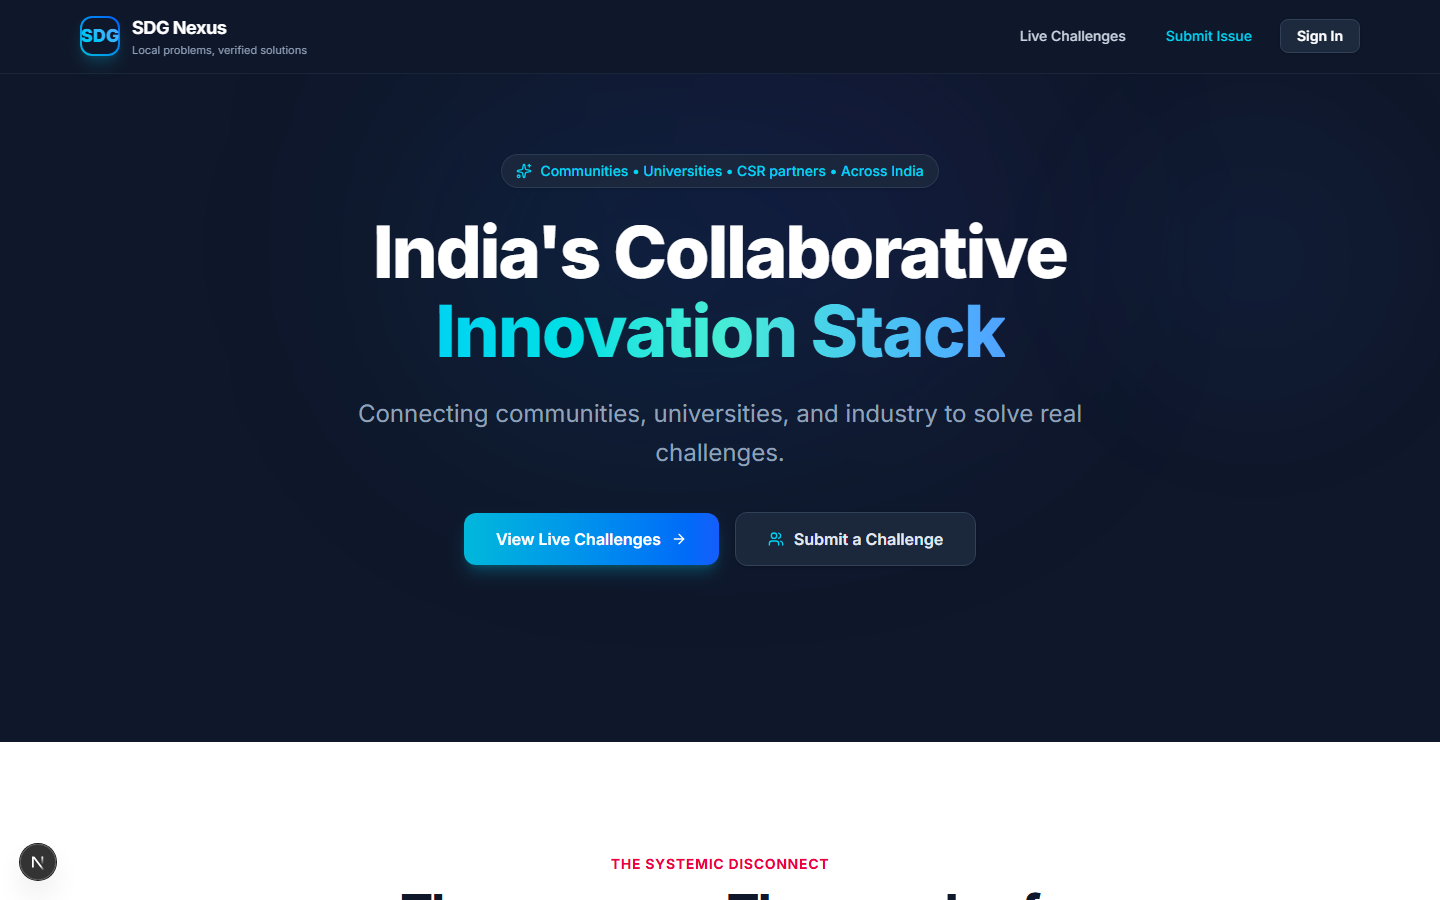
\includegraphics[width=0.92\textwidth]{figures/ui-landing.png}
\caption{Landing page of the prototype}
\label{fig:ui-landing}
\end{figure}

\begin{figure}[H]
\centering
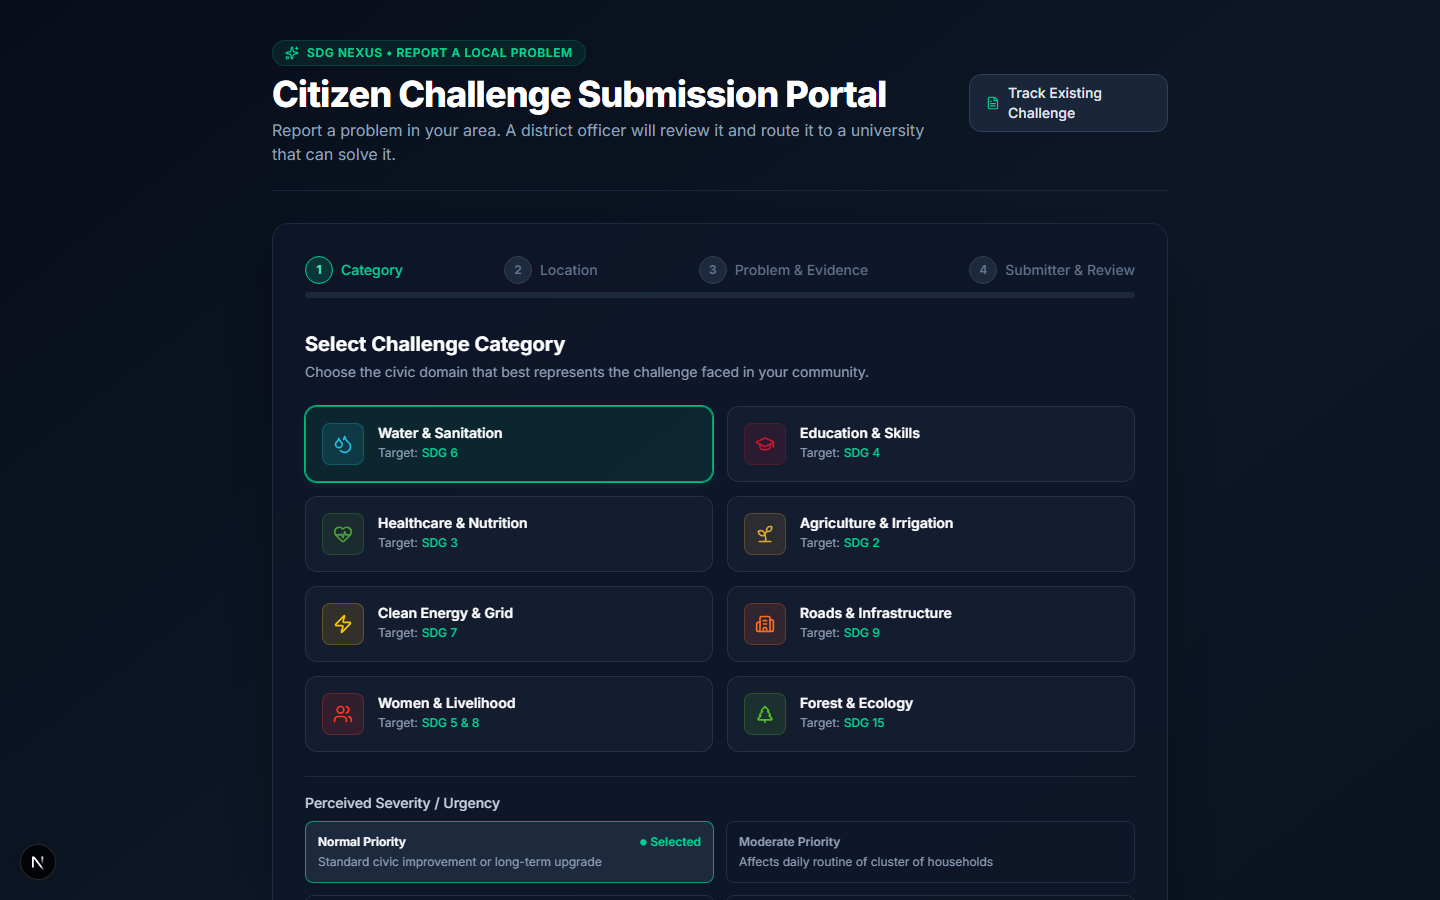
\includegraphics[width=0.92\textwidth]{figures/ui-report.png}
\caption{Citizen problem-report form (step 1: category and urgency)}
\label{fig:ui-report}
\end{figure}

\section{Innovation}
SDG Nexus introduces the following contributions:
\begin{itemize}
  \item \textbf{A citizen-closed loop.} The same citizen who reports a problem confirms (or disputes) the solution, and that confirmation feeds both the students' credentials and the organisations' impact scores. No reviewed platform closes this loop.
  \item \textbf{Money that follows proof.} Milestone amounts must add up to the budget, and each tranche can be released only after its milestone is verified, enforced inside a database transaction rather than by convention.
  \item \textbf{Server-governed lifecycle.} A single state machine on the server decides which actions are possible and returns them to the interface, so buttons cannot appear for actions that are not allowed, and every transition writes its ledger entry and notifications atomically.
  \item \textbf{Tamper evidence without a blockchain.} A per-challenge SHA-256 hash chain and server-side hashing of proof files let anyone verify the full history, at a fraction of the cost and complexity of a blockchain.
  \item \textbf{Endorsements instead of duplicates.} Repeated reports of the same problem become a measured demand signal that raises the challenge's priority instead of cluttering the officer's queue.
  \item \textbf{Explainable automation.} Priority, matching and duplicate detection are transparent formulas whose components are shown to the user, so that officers can trust and override them.
  \item \textbf{Honest by construction.} The platform never substitutes demonstration data for missing records and never reports success for an action that was not saved, a property verified by the audit and the tests above.
\end{itemize}

\chapter{Conclusion \& Future Scope}

\section{Conclusion}
SDG Nexus addresses a practical gap in how local development problems are solved in India. Citizens can report problems, universities have the talent to design solutions, companies have mandatory CSR budgets, and district officers have the authority to verify---but existing systems connect at most two of these groups and stop short of proving that a problem was actually solved.

This project designed a platform in which a single challenge record carries a problem from a citizen's report, through official verification, explainable university matching, a costed student proposal, CSR co-funding and milestone-by-milestone verification, to the same citizen's confirmation. Three ideas give the design its integrity: a server-side state machine that alone decides which actions are possible; funding that is released only against verified milestones; and a SHA-256 hash-chained ledger that lets anyone check that the recorded history has not been altered. Student credentials and organisational impact scores are derived only from this verified history.

On the implementation side, the audit of the original prototype showed that a working-looking interface can hide fabricated data, false success messages and wrong-record defects. The completed hardening phase removed every fabricated fallback, corrected the integrity, permission and privacy defects, reduced the API from 103 to 34 route files and the source tree from 199 to 111 files, and added automated integrity tests that pass in full. A duplicate-detection experiment showed that the original similarity threshold misses reworded duplicates, which led to the combined text-and-distance rule in the final design. The remaining phases build the complete lifecycle on this cleaned foundation.

\section{Future Scope}
The immediate work follows the development plan in Chapter~4: real authentication and the India-wide data model (Phase~1), the lifecycle service and ledger (Phase~2), proposals, funding and milestones (Phase~3), closure, credentials and scores (Phase~4), demonstration data and tests (Phase~5), the new interface design (Phase~6), and deployment (Phase~7). Beyond the scope of this minor project, the following extensions are possible:
\begin{itemize}
  \item \textbf{Payment integration.} Connecting funding commitments and tranche releases to a payment gateway or bank escrow, so that the recorded release and the actual transfer are the same event.
  \item \textbf{Government identity and document services.} Using DigiLocker for issuing student credentials and Aadhaar-based or e-mail/OTP verification for reporters.
  \item \textbf{Multilingual and voice reporting.} Hindi and regional-language interfaces and voice-to-text reporting, so that citizens with limited literacy can report problems.
  \item \textbf{Mobile application with offline support.} Capturing photographs and location in areas with poor connectivity and synchronising later.
  \item \textbf{Learning-based classification.} Training an SDG classifier and a duplicate detector on the platform's own verified data, once enough labelled reports exist, while keeping the current transparent methods as a fallback.
  \item \textbf{Open data.} Publishing anonymised, aggregated challenge and outcome data so that researchers and policymakers can study what kinds of local problems are solved fastest and at what cost.
  \item \textbf{Public anchoring of ledger roots.} Periodically publishing the ledger's root hashes in an external public record, so that even the platform operator could not rewrite history unnoticed.
\end{itemize}

% References in the numbered style of the prescribed format ("1. Author ...").
\makeatletter
\renewcommand{\@biblabel}[1]{#1.}
\makeatother
\renewcommand{\bibname}{REFERENCES}
\cleardoublepage
\phantomsection
\addcontentsline{toc}{chapter}{References}
\begin{thebibliography}{99}
\setlength{\itemsep}{3pt}

\bibitem{un2015} United Nations General Assembly. (2015). \emph{Transforming our world: the 2030 Agenda for Sustainable Development} (Resolution A/RES/70/1). United Nations.

\bibitem{niti2024} NITI Aayog. (2024). \emph{SDG India Index 2023--24}. Government of India.

\bibitem{companiesact2013} Government of India. (2013). \emph{The Companies Act, 2013}, Section 135: Corporate Social Responsibility. Ministry of Corporate Affairs.

\bibitem{csrrules2014} Ministry of Corporate Affairs. (2014). \emph{Companies (Corporate Social Responsibility Policy) Rules, 2014}. Government of India.

\bibitem{nep2020} Ministry of Education. (2020). \emph{National Education Policy 2020}. Government of India.

\bibitem{cpgrams} Department of Administrative Reforms and Public Grievances. \emph{Centralized Public Grievance Redress and Monitoring System (CPGRAMS)}. Government of India. https://pgportal.gov.in

\bibitem{fixmystreet} mySociety. \emph{FixMyStreet}. https://www.fixmystreet.com

\bibitem{csrportal} Ministry of Corporate Affairs. \emph{National CSR Portal}. Government of India. https://www.csr.gov.in

\bibitem{ngodarpan} NITI Aayog. \emph{NGO Darpan}. Government of India. https://ngodarpan.gov.in

\bibitem{sih} Ministry of Education's Innovation Cell and AICTE. \emph{Smart India Hackathon}. https://www.sih.gov.in

\bibitem{etzkowitz2000} Etzkowitz, H., \& Leydesdorff, L. (2000). The dynamics of innovation: from National Systems and ``Mode 2'' to a Triple Helix of university--industry--government relations. \emph{Research Policy}, 29(2), 109--123.

\bibitem{salton1988} Salton, G., \& Buckley, C. (1988). Term-weighting approaches in automatic text retrieval. \emph{Information Processing \& Management}, 24(5), 513--523.

\bibitem{sinnott1984} Sinnott, R. W. (1984). Virtues of the Haversine. \emph{Sky and Telescope}, 68(2), 159.

\bibitem{haber1991} Haber, S., \& Stornetta, W. S. (1991). How to time-stamp a digital document. \emph{Journal of Cryptology}, 3(2), 99--111.

\bibitem{merkle1987} Merkle, R. C. (1987). A digital signature based on a conventional encryption function. In \emph{Advances in Cryptology -- CRYPTO '87}, Lecture Notes in Computer Science, vol.~293, 369--378. Springer.

\bibitem{fips180} National Institute of Standards and Technology. (2015). \emph{Secure Hash Standard (SHS)}, FIPS PUB 180-4.

\bibitem{rfc7519} Jones, M., Bradley, J., \& Sakimura, N. (2015). \emph{JSON Web Token (JWT)}. RFC 7519, Internet Engineering Task Force.

\bibitem{provos1999} Provos, N., \& Mazi\`eres, D. (1999). A future-adaptable password scheme. In \emph{Proceedings of the USENIX Annual Technical Conference}, FREENIX Track.

\bibitem{owasp2021} OWASP Foundation. (2021). \emph{OWASP Top 10:2021}. https://owasp.org/Top10/

\bibitem{nextjs} Vercel. \emph{Next.js Documentation}. https://nextjs.org/docs

\bibitem{prisma} Prisma Data, Inc. \emph{Prisma ORM Documentation}. https://www.prisma.io/docs

\end{thebibliography}


\end{document}
